\documentclass[totpages,helvetica,openbib,italian]{europecv}
\usepackage[T1]{fontenc}
\usepackage{graphicx}
\usepackage[a4paper,top=1.27cm,left=1cm,right=1cm,bottom=2cm]{geometry}
\usepackage[italian]{babel}
\usepackage{bibentry}
\usepackage{url}

%\renewcommand{\ttdefault}{phv} % Uses Helvetica instead of fixed width font
\renewcommand{\normalsize}{\fontsize{9}{2}\selectfont}

\ecvname{Diego Russo}
\ecvaddress{Via G. Garibaldi 40, 05021, Acquasparta (TR), Italia}
\ecvtelephone[+39 334 5873886]{+39 0744 930614}
\ecvemail{\url{diegor.it@gmail.com} - Personale, gtalk, MSN \\& \url{diego.russo@forinicom.it} - Forinicom S.r.l.}
\ecvhomepage{\url{http://www.diegor.it}}
\ecvnationality{Italiana}
\ecvdateofbirth{30 aprile 1983}
\ecvgender{Maschio}
% \ecvbeforepicture{\raggedleft}
% \ecvpicture[width=3cm]{io}
% \ecvafterpicture{\ecvspace{-3.5cm}} 
\ecvfootnote{Per ulteriori informazioni: \url{http://europass.cedefop.eu.int}\\
\textcopyright~European Communities, 2003.}

\begin{document}
    \begin{center}
        \hspace{1pt}
        \vspace{2cm}
    
        {\scshape \textbf{\Huge Diego Russo}}
    
        \vspace{1cm}
    
        {\scshape \textbf{\large \underline{Curriculum Vitae}}}
    
        \vspace{0.25cm}
    
        aggiornato al \emph{\textbf{10 marzo 2010}}
        
        \vspace{2cm}
        
        \begin{figure}[htbp] 
            \begin{center} 
                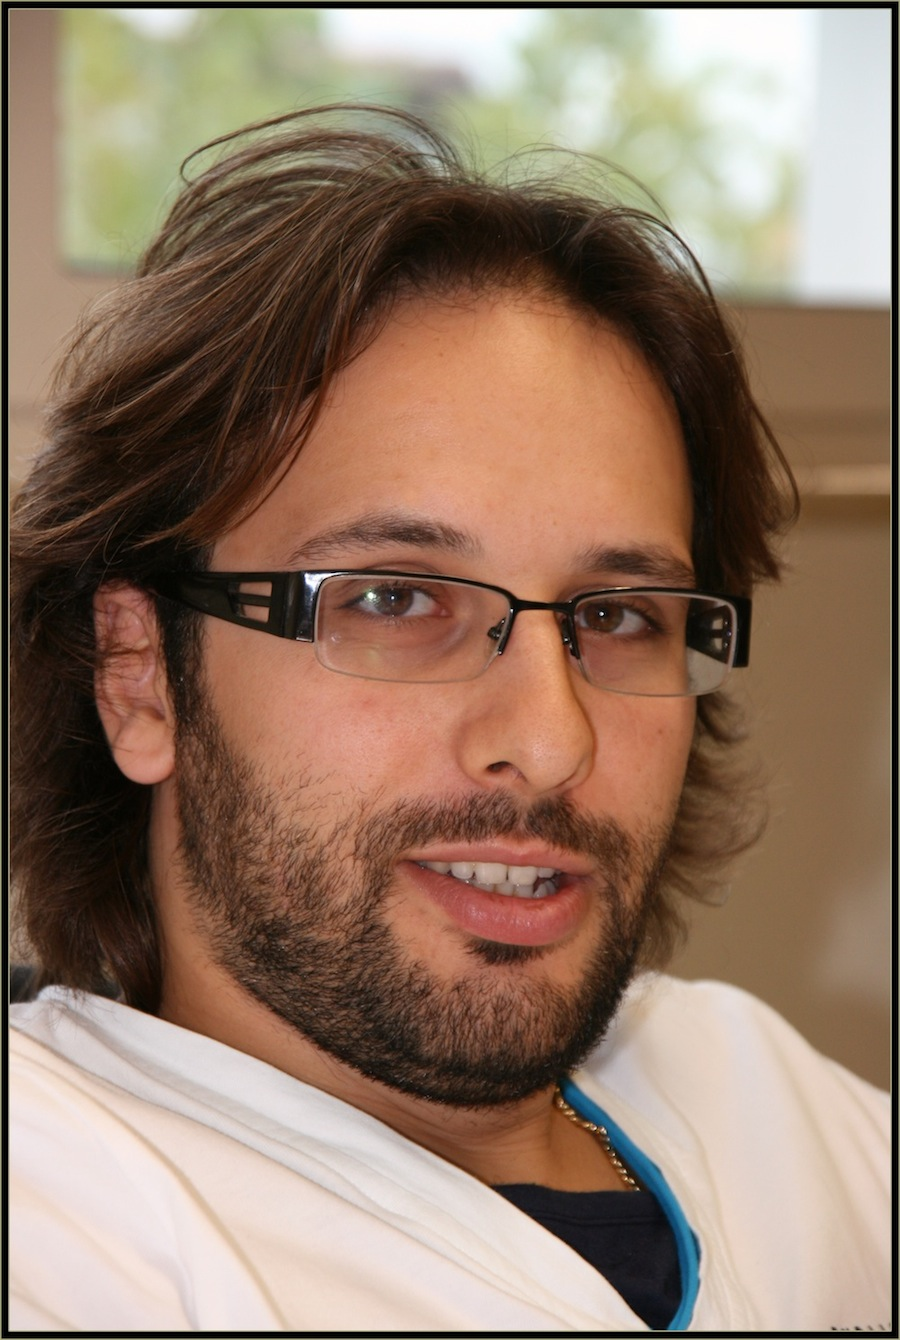
\includegraphics[width=10cm]{io.jpg}
            \end{center} 
        \end{figure}
        
    \end{center}
\pagebreak
\selectlanguage{italian}

\begin{europecv}
\ecvpersonalinfo[5pt]

%\ecvitem{\large\textbf{Impiego ricercato/ Settore di competenza}}{\large\textbf{Programmatore Python, Django.}}

\ecvsection{Esperienza professionale}

\ecvitem{Date}{\textbf{Dal 26 aprile 2008 ad Oggi}}
\ecvitem{Lavoro o posizione ricoperti}{Programmatore, sistemista (lavoratore con contratto di apprendistato part-time, 25 ore)}
\ecvitem{Principali attivit\'a e responsabilit\`a}{Sviluppo di un progetto che mira ad offrire connettivit\'a e servizi integrati (videosorveglianza, voip) alle pubbliche amministrazioni, aziende e privati. Punti previsti dal contratto:
\begin{itemize}
    \item conoscere i prodotti ed i servizi del settore e del contesto aziendale: reti Mesh e gararchiche, servizi VoIP e videosorveglianza, sicurezza delle reti wired e wireless;
    \item conoscere e saper applicare le basi tecniche e scientifiche della professionalit\'a;
    \item conoscere e saper utilizzare tecniche e metodi di lavoro con particolare riferimento allo sviluppo software e alla documentazione del codice;
    \item conoscere e saper utilizzare strumenti e tecnologie di lavoro (attrezzature, macchinari e strumenti di lavoro), in particolare ambiente di sviluppo Linux, piattaforma di sviluppo Linux/OSX, linguaggi di programmazione Python e database PostgresSQL/MySQL;
    \item conoscere ed utilizzare misure di sicurezza individuale e per la tutela ambientale;
    \item conoscere le innovazioni di prodotto, di processo, di contesto e di settore.
\end{itemize}
Inoltre ho sviluppato applicazioni in python e in python-django sia per il lavoro quotidiano del reparto tecnico e non sia di pura ricerca e sviluppo. A tal senso ho implementato da zero un server per gestire il \textbf{servizio di hotspot}.}
\ecvitem{Nome e indirizzo del datore di lavoro}{Forinicom srl, Via del Popolo, 9 Bastia Umbra, 06083, 0758001868, \url{http://www.forinicom.it}}
\ecvitem{Tipo di attivit\`a o settore}{Settore telecomunicazioni}

\ecvitem[15pt]{}{}

\ecvitem{Date}{\textbf{Dal 03 settembre 2009 ad Oggi}}
\ecvitem{Lavoro o posizione ricoperti}{Programmatore (lavoratore con contratto a progetto, part-time)}
\ecvitem{Principali attivit\'a e responsabilit\`a}{Sviluppo di un'applicazione gestionale per il comune di Bettona in django, python, postgresql, linux, apache, per l'informatizzazione dei servizi per la gestione delle anagrafiche nonch\'e delle pratiche edilizie ed urbanistiche e del calcolo della tassa ICI con aggiornamenti dei dati catastali. Utilizzo di un server per il controllo di versione (GIT). Inoltre in questa fase c'\'e stata il completamento del prodotto con la relativa commercializzazione.}
\ecvitem{Nome e indirizzo del datore di lavoro}{Consorzio Miles - Servizi Integrati, CF 04881101002, Via Rocca di Papa 21, Roma}
\ecvitem{Tipo di attivit\`a o settore}{Servizi integrati per la pubblica amministrazione}

\ecvitem[15pt]{}{}

\ecvitem{Date}{\textbf{Dal 01 agosto 2007 al 31 agosto 2008}}
\ecvitem{Lavoro o posizione ricoperti}{Programmatore (lavoratore con contratto a progetto, full-time)}
\ecvitem{Principali attivit\'a e responsabilit\`a}{Sviluppo di un'applicazione gestionale per il comune di Bettona in django, python, postgresql, linux, apache, per l'informatizzazione dei servizi per la gestione delle anagrafiche nonch\'e delle pratiche edilizie ed urbanistiche e del calcolo della tassa ICI con aggiornamenti dei dati catastali. Utilizzo di un server per il controllo di versione (SVN), con relativa interfaccia web (trac) per la gestione dei ticket.}
\ecvitem{Nome e indirizzo del datore di lavoro}{Consorzio Miles - Servizi Integrati, CF 04881101002, Via Rocca di Papa 21, Roma}
\ecvitem{Tipo di attivit\`a o settore}{Servizi integrati per la pubblica amministrazione}

\ecvitem[15pt]{}{}

\ecvitem{Date}{\textbf{Dal 11 dicembre 2006 al 30 luglio 2007}}
\ecvitem{Lavoro o posizione ricoperti}{Programmatore (lavoratore con contratto a progetto, full-time)}
\ecvitem{Principali attivit\'a e responsabilit\`a}{Sviluppo di un'applicazione gestionale per il comune di Bettona in django, python, postgresql, linux, apache, per l'informatizzazione dei servizi per la gestione delle anagrafiche nonch\'e delle pratiche edilizie ed urbanistiche e del calcolo della tassa ICI con aggiornamenti dei dati catastali. Utilizzo di un server per il controllo di versione (SVN), con relativa interfaccia web (trac) per la gestione dei ticket.}
\ecvitem{Nome e indirizzo del datore di lavoro}{Consorzio Miles - Servizi Integrati, CF 04881101002, Via Rocca di Papa 21, Roma}
\ecvitem{Tipo di attivit\`a o settore}{Servizi integrati per la pubblica amministrazione}

\ecvitem[15pt]{}{}

\ecvitem{Date}{\textbf{Dal 30 luglio 2006 al 30 dicembre 2006}}
\ecvitem{Lavoro o posizione ricoperti}{Tesista (Wireless Broadband Network)}
\ecvitem{Principali attivit\'a e responsabilit\`a}{Wireless Broadband Network - progetto \textbf{WeConnect} - Banda larga su reti wireless:
    \begin{itemize}
        \item Ampia conoscenza della rete wireless e del suo funzionamento
        \item Buona conoscenza della normativa che regola il Wi-Fi
        \item Ottima conoscenza del sistema RouterOS (www.mikrotik.com)
        \item Conoscenza del protocollo AAA e del server FreeRADIUS
        \item Amministrazione dei vari servizi di rete: mail (postfix), server web (apache), DNS (pdns), firewall (iptables), database (postgresql), hotspot (chillispot), OS Debian, Voyage (OS per sistemi embedded, basata su Debian)
    \end{itemize} 
}
\ecvitem{Nome e indirizzo del datore di lavoro}{WEDOIT s.a.s. - Via Protomartiri Francescani,26 - 06088 Assisi (PG)}
\ecvitem{Tipo di attivit\`a o settore}{Soluzioni informatiche}

\ecvitem[15pt]{}{}

\ecvitem{Date}{\textbf{Dal 14 novembre 2005 al 30 maggio 2006}}
\ecvitem{Lavoro o posizione ricoperti}{Stagista (S.E.O. Search Engine Optimization)}
\ecvitem{Principali attivit\'a e responsabilit\`a}{
    \begin{itemize}
        \item Conoscenza del SEO e dei sui meccanismi. Ottimizzazione di un sito per il S.E.O.
        \item Tecniche di Pageranking e link popularity
        \item Sistemista di un server virtuale, basato su Debian
        \item Apprendimento del linguaggio di programmazione Python
    \end{itemize}
}
\ecvitem{Nome e indirizzo del datore di lavoro}{WEDOIT s.a.s. - Via Protomartiri Francescani,26 - 06088 Assisi (PG)}
\ecvitem{Tipo di attivit\`a o settore}{Soluzioni informatiche}

\ecvitem[15pt]{}{}

\ecvitem{Date}{\textbf{Marzo 2002}}
\ecvitem{Lavoro o posizione ricoperti}{Stagista (Stage abbinato al progetto IFS, Impresa Formativa Simulata)}
\ecvitem{Principali attivit\'a e responsabilit\`a}{Gestione della rete interna dell'impresa}
\ecvitem{Nome e indirizzo del datore di lavoro}{IOSA CARLO S.r.l. - 05100 TERNI - Via Pallotta n. 7 - Tel. (0744) 2460 - Fax (0744) 246035 - P.IVA 00072550551 - \url{http://www.iosacarlo.com} - \url{iosacarlo@iosacarlo.com}}
\ecvitem{Tipo di attivit\`a o settore}{Impresa smaltimento rifiuti}

\ecvitem[15pt]{}{} 















\ecvsection{Istruzione e formazione}

\ecvitem{Date}{Iniziare con le informazioni pi\'u recenti ed elencare separatamente ciascun corso frequentato con successo. Facoltativo.}
\ecvitem{Certificato o diploma ottenuto}{\ldots}
\ecvitem{Principali materie/Competenze professionali apprese}{\ldots}
\ecvitem{Nome e tipo d'istituto di istruzione o formazione}{\ldots}
\ecvitem{Livello nella classificazione nazionale o internazionale\footnote{Se pertinente.}}{\ldots}

\ecvsection{Capacit\`a e competenze professionali}

\ecvmothertongue[80pt]{Precisare madrelingua/e}
\ecvitem{\large Altra/e lingua/e}{}
\ecvlanguageheader{(*)}
\ecvlanguage{Lingua}{\ecvAOne}{\ecvAOne}{\ecvATwo}{\ecvCOne}{\ecvCOne}
\ecvlastlanguage{Lingua}{\ecvCOne}{\ecvCOne}{}{}{\ecvCTwo}
\ecvlanguagefooter[10pt]{(*)}

\ecvitem[10pt]{Capacit\`a e competenze sociali}{Descrivere tali competenze e indicare dove sono state acquisite. Facoltativo.}
\ecvitem[10pt]{Capacit\`a e competenze organizzative}{Descrivere tali competenze e indicare dove sono state acquisite. Facoltativo.}
\ecvitem[10pt]{Capacit\`a e competenze tecniche}{Descrivere tali competenze e indicare dove sono state acquisite. Facoltativo.}
\ecvitem[10pt]{Capacit\`a e competenze informatiche}{Descrivere tali competenze e indicare dove sono state acquisite. Facoltativo.}
\ecvitem[10pt]{Capacit\`a e competenze artistiche}{Descrivere tali competenze e indicare dove sono state acquisite. Facoltativo.}
\ecvitem[10pt]{Altre capacit\`a e competenze}{Descrivere tali competenze e indicare dove sono state acquisite. Facoltativo.}
\ecvitem{Patente/i}{Indicare la(e) patente(i) di cui siete titolari precisandone la categoria. Facoltativo.}

\ecvsection{Ulteriori informazioni}
\ecvitem[10pt]{}{Inserire qui ogni altra informazione utile, ad esempio persone di riferimento, referenze, etc\ldots Facoltativo.}
\bibliographystyle{plain}
\nobibliography{publications}
% \ecvitem{}{\textbf{Pubblicazioni}}
% \ecvitem{}{\bibentry{pub1}}
% \ecvitem[10pt]{}{\bibentry{pub2}}
% \ecvitem{}{\textbf{Interessi personali}}
% \ecvitem{}{\ldots}  

\ecvsection{Allegati}
\ecvitem{}{Enumerare gli allegati al CV.}
\end{europecv}


\end{document} 